%%%%%%%%%%%%%%%%%%%%%%%%%%%%%%%%%%%%%%%%%%%%%%%%%%%%%%%%%%%%%%%%%%%%%%%%%%%%%%%%
% Modelo para apresentações do Magister
%
% Por: Abrantes Araújo Silva Filho
%      abrantesasf@gmail.com


%%%%%%%%%%%%%%%%%%%%%%%%%%%%%%%%%%%%%%%%%%%%%%%%%%%%%%%%%%%%%%%%%%%%%%%%%%%%%%%%
%%% Classe do documento
\RequirePackage{ifpdf}
\ifpdf
  \pdfminorversion=7
  \documentclass[pdftex, brazil, aspectratio=169]{beamer}
\else
  \documentclass[brazil, aspectratio=169]{beamer}
\fi
\setbeamertemplate{navigation symbols}{}
\usetheme{Magister}
\usefonttheme[onlymath]{serif}


%%%%%%%%%%%%%%%%%%%%%%%%%%%%%%%%%%%%%%%%%%%%%%%%%%%%%%%%%%%%%%%%%%%%%%%%%%%%%%%%
%%% Preâmbulo com todas as outras outras chamadas para todos os outros packages
%%% e o que mais for necessário
%%%%%%%%%%%%%%%%%%%%%%%%%%%%%%%%%%%%%%%%%%%%%%%%%%%%%%%%%%%%%%%%%%%%%%%%%%%%%%%%
% Por: Abrantes Araújo Silva Filho
%      abrantesasf@gmail.com
% URL: https://github.com/abrantesasf/latex


%%%%%%%%%%%%%%%%%%%%%%%%%%%%%%%%%%%%%%%%%%%%%%%%%%%%%%%%%%%%%%%%%%%%%%%%%%%%%%%%
%%% Compilação condicional em PDF
%%%%%%%%%%%%%%%%%%%%%%%%%%%%%%%%%%%%%%%%%%%%%%%%%%%%%%%%%%%%%%%%%%%%%%%%%%%%%%%%
% Por: Abrantes Araújo Silva Filho
%      abrantesasf@gmail.com
% URL: https://github.com/abrantesasf/latex


%%%%%%%%%%%%%%%%%%%%%%%%%%%%%%%%%%%%%%%%%%%%%%%%%%%%%%%%%%%%%%%%%%%%%%%%%%%%%%%%
%%% Pacote para compilaçãocondicional em PDF
\usepackage{ifpdf}


%%%%%%%%%%%%%%%%%%%%%%%%%%%%%%%%%%%%%%%%%%%%%%%%%%%%%%%%%%%%%%%%%%%%%%%%%%%%%%%%
%%% Estruturas de controle
%%%%%%%%%%%%%%%%%%%%%%%%%%%%%%%%%%%%%%%%%%%%%%%%%%%%%%%%%%%%%%%%%%%%%%%%%%%%%%%%
% Por: Abrantes Araújo Silva Filho
%      abrantesasf@gmail.com
% URL: https://github.com/abrantesasf/latex


%%%%%%%%%%%%%%%%%%%%%%%%%%%%%%%%%%%%%%%%%%%%%%%%%%%%%%%%%%%%%%%%%%%%%%%%%%%%%%%%
%%% Carrega pacotes iniciais necessários para estrutura de controle e para a
%%% criação e o parse de novos comandos
\usepackage{ifthen}
\usepackage{xparse}



%%%%%%%%%%%%%%%%%%%%%%%%%%%%%%%%%%%%%%%%%%%%%%%%%%%%%%%%%%%%%%%%%%%%%%%%%%%%%%%%
%%% Configurações de layout da página
%%%%%%%%%%%%%%%%%%%%%%%%%%%%%%%%%%%%%%%%%%%%%%%%%%%%%%%%%%%%%%%%%%%%%%%%%%%%%%%%
% Por: Abrantes Araújo Silva Filho
%      abrantesasf@gmail.com
% URL: https://github.com/abrantesasf/latex


%%%%%%%%%%%%%%%%%%%%%%%%%%%%%%%%%%%%%%%%%%%%%%%%%%%%%%%%%%%%%%%%%%%%%%%%%%%%%%%%
%%% Configuração do tamanho da página, margens, espaçamento entrelinhas e, se
%%% necessário, ativa a indentação dos primeiros parágrafos.
\makeatletter
\@ifclassloaded{beamer}{}{
\ifpdf
  \usepackage[pdftex]{geometry}
\else
  \usepackage[dvips]{geometry}
\fi
}
\makeatother

\usepackage{setspace}


%%%%%%%%%%%%%%%%%%%%%%%%%%%%%%%%%%%%%%%%%%%%%%%%%%%%%%%%%%%%%%%%%%%%%%%%%%%%%%%%
%%% Cabeçalho e rodapé
%%%%%%%%%%%%%%%%%%%%%%%%%%%%%%%%%%%%%%%%%%%%%%%%%%%%%%%%%%%%%%%%%%%%%%%%%%%%%%%%%
% Por: Abrantes Araújo Silva Filho
%      abrantesasf@gmail.com
% URL: https://github.com/abrantesasf/latex


%%%%%%%%%%%%%%%%%%%%%%%%%%%%%%%%%%%%%%%%%%%%%%%%%%%%%%%%%%%%%%%%%%%%%%%%%%%%%%%%
%%% Configurações de cabeçalho e rodapé:
%%% Atenção: é MUITO DIFÍCIL ajustar apropriadamente os running header
%%% e footer da primeira vez. Você pode confiar no LaTeX e deixar que
%%% ele faça o ajuste automaticamente ou pode quebrar a cabeça e
%%% tentar melhorar algo que o LaTeX já faz muito bem. O que você
%%% perfere?
\usepackage{fancyhdr}
\setlength{\headheight}{1cm}
\setlength{\footskip}{1.5cm}
\renewcommand{\headrulewidth}{0.3pt}
\renewcommand{\footrulewidth}{0.0pt}
\pagestyle{fancy}
\renewcommand{\sectionmark}[1]{%
  \markboth{\uppercase{#1}}{}}
\renewcommand{\subsectionmark}[1]{%
  \markright{\uppercase{\thesubsection \hspace{0.1cm} #1}}{}}
\fancyhead{}
\fancyfoot{}
\newcommand{\diminuifonte}{%
    \fontsize{9pt}{9}\selectfont
}
\newcommand{\aumentafonte}{%
    \fontsize{12}{12}\selectfont
}
% Configura cabeçalho e rodapé para documentos TWOSIDE
\fancyhead[EL]{\textbf{\thepage}}
\fancyhead[EC]{}
\fancyhead[ER]{\diminuifonte \textbf{\leftmark}}
\fancyhead[OR]{\textbf{\thepage}}
\fancyhead[OC]{}
\fancyhead[OL]{\diminuifonte \textbf{\rightmark}}
\fancyfoot[EL,EC,ER,OR,OC,OL]{}
% Configura cabeçalho e rodapé para documentos ONESIDE
%%\lhead{ \fancyplain{}{sup esquerdo} }
%%\chead{ \fancyplain{}{sup centro} }
%%\rhead{ \fancyplain{}{\thesection} }
%%\lfoot{ \fancyplain{}{inf esquerdo} }
%%\cfoot{ \fancyplain{}{inf centro} }
%%\rfoot{ \fancyplain{}{\thepage} }


%%%%%%%%%%%%%%%%%%%%%%%%%%%%%%%%%%%%%%%%%%%%%%%%%%%%%%%%%%%%%%%%%%%%%%%%%%%%%%%%
%%% Fontes
%%%%%%%%%%%%%%%%%%%%%%%%%%%%%%%%%%%%%%%%%%%%%%%%%%%%%%%%%%%%%%%%%%%%%%%%%%%%%%%%
% Por: Abrantes Araújo Silva Filho
%      abrantesasf@gmail.com
% URL: https://github.com/abrantesasf/latex


%%%%%%%%%%%%%%%%%%%%%%%%%%%%%%%%%%%%%%%%%%%%%%%%%%%%%%%%%%%%%%%%%%%%%%%%%%%%%%%%
%%% Configurações de encoding, lingua e fontes:
\usepackage[T1]{fontenc}
\usepackage[utf8]{inputenc}

% Altera a fonte padrão do documento (nem todas funcionam em modo math):
%   phv = Helvetica
%   ptm = Times
%   ppl = Palatino
%   pbk = bookman
%   pag = AdobeAvantGarde
%   pnc = Adobe NewCenturySchoolBook
\renewcommand{\familydefault}{ppl}


%%%%%%%%%%%%%%%%%%%%%%%%%%%%%%%%%%%%%%%%%%%%%%%%%%%%%%%%%%%%%%%%%%%%%%%%%%%%%%%%
%%% Linguagem e hifenização
%%%%%%%%%%%%%%%%%%%%%%%%%%%%%%%%%%%%%%%%%%%%%%%%%%%%%%%%%%%%%%%%%%%%%%%%%%%%%%%%
% Por: Abrantes Araújo Silva Filho
%      abrantesasf@gmail.com
% URL: https://github.com/abrantesasf/latex


%%%%%%%%%%%%%%%%%%%%%%%%%%%%%%%%%%%%%%%%%%%%%%%%%%%%%%%%%%%%%%%%%%%%%%%%%%%%%%%%
%%% Configurações de linguagem e hifenização
\usepackage[brazil]{babel}

%%%%%%%%%%%%%%%%%%%%%%%%%%%%%%%%%%%%%%%%%%%%%%%%%%%%%%%%%%%%%%%%%%%%%%%%%%%%%%%%
%%% Hifenização específica quando o LaTeX/Babel não conseguirem hifenizar:
\babelhyphenation{Git-Hub}


%%%%%%%%%%%%%%%%%%%%%%%%%%%%%%%%%%%%%%%%%%%%%%%%%%%%%%%%%%%%%%%%%%%%%%%%%%%%%%%%
%%% Matemática
%%%%%%%%%%%%%%%%%%%%%%%%%%%%%%%%%%%%%%%%%%%%%%%%%%%%%%%%%%%%%%%%%%%%%%%%%%%%%%%%
% Por: Abrantes Araújo Silva Filho
%      abrantesasf@gmail.com
% URL: https://github.com/abrantesasf/latex


%%%%%%%%%%%%%%%%%%%%%%%%%%%%%%%%%%%%%%%%%%%%%%%%%%%%%%%%%%%%%%%%%%%%%%%%%%%%%%%%
%%% Carrega bibliotecas e símbolos matemáticos, fontes adicionais e configura
%%% algumas outras opções
\usepackage{amsmath}
\usepackage{amssymb}
\usepackage{amsthm}
\usepackage{amsfonts}
\usepackage{siunitx}
  \sisetup{group-separator = {.}}
  \sisetup{group-digits = {true}}
  \sisetup{output-decimal-marker = {,}}
\usepackage{bm}
\usepackage{cancel}

% Altera separador decimal via comando, se necessário (prefira o siunitx):
%\mathchardef\period=\mathcode`.
%\DeclareMathSymbol{.}{\mathord}{letters}{"3B}

\usepackage{esvect}
\usepackage{mathtools}

%%%%%%%%%%%%%%%%%%%%%%%%%%%%%%%%%%%%%%%%%%%%%%%%%%%%%%%%%%%%%%%%%%%%%%%%%%%%%%%%
%%% Definições para teoremas, etc.
\makeatletter
\@ifclassloaded{article}{
\theoremstyle{definition}
\newtheorem{definicao}{Definição}[section]
\newtheorem{conjecture}{Conjectura}[section]
\newtheorem{teorema}{Teorema}[section]
\newtheorem{lemma}{Lema}[section]
\newtheorem{corolario}{Corolario}[section]
\theoremstyle{remark}
\newtheorem*{nota}{Nota}
\newtheorem*{observacao}{Observação:}
}{}
\@ifclassloaded{book}{
\theoremstyle{definition}
\newtheorem{definicao}{Definição}[chapter]
\newtheorem{conjecture}{Conjectura}[chapter]
\newtheorem{teorema}{Teorema}[chapter]
\newtheorem{lemma}{Lema}[chapter]
\newtheorem{corolario}{Corolario}[chapter]
\theoremstyle{remark}
\newtheorem*{nota}{Nota}
\newtheorem*{observacao}{Observação:}
}{}
\makeatother


%%%%%%%%%%%%%%%%%%%%%%%%%%%%%%%%%%%%%%%%%%%%%%%%%%%%%%%%%%%%%%%%%%%%%%%%%%%%%%%%
%%% Sumário
%%%%%%%%%%%%%%%%%%%%%%%%%%%%%%%%%%%%%%%%%%%%%%%%%%%%%%%%%%%%%%%%%%%%%%%%%%%%%%%%
% Por: Abrantes Araújo Silva Filho
%      abrantesasf@gmail.com
% URL: https://github.com/abrantesasf/latex


%%%%%%%%%%%%%%%%%%%%%%%%%%%%%%%%%%%%%%%%%%%%%%%%%%%%%%%%%%%%%%%%%%%%%%%%%%%%%%%%
%%% Ajustes de sumário
\makeatletter
\@ifclassloaded{article}{
\usepackage[nottoc]{tocbibind}
}{}
\@ifclassloaded{book}{
\usepackage{tocbibind}
}{}
\makeatother


%%%%%%%%%%%%%%%%%%%%%%%%%%%%%%%%%%%%%%%%%%%%%%%%%%%%%%%%%%%%%%%%%%%%%%%%%%%%%%%%
%%% Referências cruzadas, links, citações
%%%%%%%%%%%%%%%%%%%%%%%%%%%%%%%%%%%%%%%%%%%%%%%%%%%%%%%%%%%%%%%%%%%%%%%%%%%%%%%%
% Por: Abrantes Araújo Silva Filho
%      abrantesasf@gmail.com
% URL: https://github.com/abrantesasf/latex


%%%%%%%%%%%%%%%%%%%%%%%%%%%%%%%%%%%%%%%%%%%%%%%%%%%%%%%%%%%%%%%%%%%%%%%%%%%%%%%%%
%%% Carrega pacotes para referências cruzadas, citações dentro do documento,
%%% links para internet e outros.Configura algumas opções.
%%% Não altere a ordem de carregamento dos packages.
\usepackage{varioref}
\ifpdf
  \usepackage[pdftex]{hyperref}
    \hypersetup{
      % Configurações padrão que eu gosto
      unicode=true,
      pdflang={pt-BR},
      bookmarksopen=true,
      bookmarksnumbered=true,
      bookmarksopenlevel=5,
      pdfdisplaydoctitle=true,
      pdfpagemode=UseOutlines,
      pdfstartview=FitH,
      pdfcreator={LaTeX with hyperref package},
      pdfproducer={pdfTeX},
      pdfnewwindow=true,
      colorlinks=true,
      citecolor=red,
      linkcolor=red,
      filecolor=cyan,
      urlcolor=blue
    }
\else
  \usepackage{hyperref}
\fi
\usepackage{cleveref}
\usepackage{url}


%%%%%%%%%%%%%%%%%%%%%%%%%%%%%%%%%%%%%%%%%%%%%%%%%%%%%%%%%%%%%%%%%%%%%%%%%%%%%%%%
%%% Referências bibliográficas
%%%%%%%%%%%%%%%%%%%%%%%%%%%%%%%%%%%%%%%%%%%%%%%%%%%%%%%%%%%%%%%%%%%%%%%%%%%%%%%%
%%% Referências bibliográficas
\usepackage[round, semicolon, authoryear]{natbib}
%\bibliographystyle{natdin}
\bibliographystyle{abrantesasf}


%%%%%%%%%%%%%%%%%%%%%%%%%%%%%%%%%%%%%%%%%%%%%%%%%%%%%%%%%%%%%%%%%%%%%%%%%%%%%%%%
%%% Glossário e índice remissivo
%%%%%%%%%%%%%%%%%%%%%%%%%%%%%%%%%%%%%%%%%%%%%%%%%%%%%%%%%%%%%%%%%%%%%%%%%%%%%%%%
%%% Pacotes para glossário e índice remissivo
\usepackage{makeidx}
\makeindex

\usepackage[toc]{glossaries}
\newglossary[nlg]{notation}{not}{ntn}{Notação}

\newglossaryentry{not:set}{
type = notation,
name = {$\mathbb{N}$},
description = conjunto dos números naturais,
sort = {N}}

\makeglossaries


%%%%%%%%%%%%%%%%%%%%%%%%%%%%%%%%%%%%%%%%%%%%%%%%%%%%%%%%%%%%%%%%%%%%%%%%%%%%%%%%
%%% Computação
%%%%%%%%%%%%%%%%%%%%%%%%%%%%%%%%%%%%%%%%%%%%%%%%%%%%%%%%%%%%%%%%%%%%%%%%%%%%%%%%
% Por: Abrantes Araújo Silva Filho
%      abrantesasf@gmail.com
% URL: https://github.com/abrantesasf/latex


%%%%%%%%%%%%%%%%%%%%%%%%%%%%%%%%%%%%%%%%%%%%%%%%%%%%%%%%%%%%%%%%%%%%%%%%%%%%%%%%
%%% Carrega packages relacionados à computação
\usepackage{algorithm2e}
\usepackage{algorithmicx}
\usepackage{algpseudocode}
\usepackage{listings}
  \lstset{literate=
    {á}{{\'a}}1 {é}{{\'e}}1 {í}{{\'i}}1 {ó}{{\'o}}1 {ú}{{\'u}}1
    {Á}{{\'A}}1 {É}{{\'E}}1 {Í}{{\'I}}1 {Ó}{{\'O}}1 {Ú}{{\'U}}1
    {à}{{\`a}}1 {è}{{\`e}}1 {ì}{{\`i}}1 {ò}{{\`o}}1 {ù}{{\`u}}1
    {À}{{\`A}}1 {È}{{\'E}}1 {Ì}{{\`I}}1 {Ò}{{\`O}}1 {Ù}{{\`U}}1
    {ä}{{\"a}}1 {ë}{{\"e}}1 {ï}{{\"i}}1 {ö}{{\"o}}1 {ü}{{\"u}}1
    {Ä}{{\"A}}1 {Ë}{{\"E}}1 {Ï}{{\"I}}1 {Ö}{{\"O}}1 {Ü}{{\"U}}1
    {â}{{\^a}}1 {ê}{{\^e}}1 {î}{{\^i}}1 {ô}{{\^o}}1 {û}{{\^u}}1
    {Â}{{\^A}}1 {Ê}{{\^E}}1 {Î}{{\^I}}1 {Ô}{{\^O}}1 {Û}{{\^U}}1
    {œ}{{\oe}}1 {Œ}{{\OE}}1 {æ}{{\ae}}1 {Æ}{{\AE}}1 {ß}{{\ss}}1
    {ű}{{\H{u}}}1 {Ű}{{\H{U}}}1 {ő}{{\H{o}}}1 {Ő}{{\H{O}}}1
    {ç}{{\c c}}1 {Ç}{{\c C}}1 {ø}{{\o}}1 {å}{{\r a}}1 {Å}{{\r A}}1
    {€}{{\euro}}1 {£}{{\pounds}}1 {«}{{\guillemotleft}}1
    {»}{{\guillemotright}}1 {ñ}{{\~n}}1 {Ñ}{{\~N}}1 {¿}{{?`}}1
  }


%%%%%%%%%%%%%%%%%%%%%%%%%%%%%%%%%%%%%%%%%%%%%%%%%%%%%%%%%%%%%%%%%%%%%%%%%%%%%%%%
%%% Cores
%%%%%%%%%%%%%%%%%%%%%%%%%%%%%%%%%%%%%%%%%%%%%%%%%%%%%%%%%%%%%%%%%%%%%%%%%%%%%%%%
% Por: Abrantes Araújo Silva Filho
%      abrantesasf@gmail.com
% URL: https://github.com/abrantesasf/latex


%%%%%%%%%%%%%%%%%%%%%%%%%%%%%%%%%%%%%%%%%%%%%%%%%%%%%%%%%%%%%%%%%%%%%%%%%%%%%%%%
%%% Ativa suporte extendido a cores
\makeatletter
\@ifclassloaded{beamer}{
  \usepackage{xcolor} % Opções de cores: usenames (16), dvipsnames (64),
                      % svgnames (150) e x11names (300).
}{
  \usepackage[svgnames]{xcolor} % Opções de cores: usenames (16), dvipsnames (64),
                                % svgnames (150) e x11names (300).
}
\makeatother


%%%%%%%%%%%%%%%%%%%%%%%%%%%%%%%%%%%%%%%%%%%%%%%%%%%%%%%%%%%%%%%%%%%%%%%%%%%%%%%%
%%% Gráficos
%%%%%%%%%%%%%%%%%%%%%%%%%%%%%%%%%%%%%%%%%%%%%%%%%%%%%%%%%%%%%%%%%%%%%%%%%%%%%%%%
% Por: Abrantes Araújo Silva Filho
%      abrantesasf@gmail.com
% URL: https://github.com/abrantesasf/latex


%%%%%%%%%%%%%%%%%%%%%%%%%%%%%%%%%%%%%%%%%%%%%%%%%%%%%%%%%%%%%%%%%%%%%%%%%%%%%%%%
%%% Suporte à importação de gráficos externos
%\usepackage{tcolorbox}
\ifpdf
  \usepackage[pdftex]{graphicx}
\else
  \usepackage[dvips]{graphicx}
\fi

%%%%%%%%%%%%%%%%%%%%%%%%%%%%%%%%%%%%%%%%%%%%%%%%%%%%%%%%%%%%%%%%%%%%%%%%%%%%%%%%
%%% Suporte à criação de gráficos proceduralmente no LaTeX:
\usepackage{tikz}
\usetikzlibrary{arrows,automata,backgrounds,matrix,patterns,positioning,shapes,shadows}



%%%%%%%%%%%%%%%%%%%%%%%%%%%%%%%%%%%%%%%%%%%%%%%%%%%%%%%%%%%%%%%%%%%%%%%%%%%%%%%%
%%% Ícones
%%%%%%%%%%%%%%%%%%%%%%%%%%%%%%%%%%%%%%%%%%%%%%%%%%%%%%%%%%%%%%%%%%%%%%%%%%%%%%%%
% Por: Abrantes Araújo Silva Filho
%      abrantesasf@gmail.com
% URL: https://github.com/abrantesasf/latex


%%%%%%%%%%%%%%%%%%%%%%%%%%%%%%%%%%%%%%%%%%%%%%%%%%%%%%%%%%%%%%%%%%%%%%%%%%%%%%%%
%%% Pacotes com ícones, figuras e gráficos extras

% Ícones da Creative Commons:
\usepackage{ccicons}


%%%%%%%%%%%%%%%%%%%%%%%%%%%%%%%%%%%%%%%%%%%%%%%%%%%%%%%%%%%%%%%%%%%%%%%%%%%%%%%%
%%% Blocos
%%%%%%%%%%%%%%%%%%%%%%%%%%%%%%%%%%%%%%%%%%%%%%%%%%%%%%%%%%%%%%%%%%%%%%%%%%%%%%%%
% Por: Abrantes Araújo Silva Filho
%      abrantesasf@gmail.com
% URL: https://github.com/abrantesasf/latex


%%%%%%%%%%%%%%%%%%%%%%%%%%%%%%%%%%%%%%%%%%%%%%%%%%%%%%%%%%%%%%%%%%%%%%%%%%%%%%%%
%%% Ambiente para boxes em posições arbitrárias

\makeatletter
\@ifclassloaded{beamer}{
  \usepackage{textpos}
}{}
\makeatother


%%%%%%%%%%%%%%%%%%%%%%%%%%%%%%%%%%%%%%%%%%%%%%%%%%%%%%%%%%%%%%%%%%%%%%%%%%%%%%%%
%%% Boxes coloridos
%%%%%%%%%%%%%%%%%%%%%%%%%%%%%%%%%%%%%%%%%%%%%%%%%%%%%%%%%%%%%%%%%%%%%%%%%%%%%%%%
% Por: Abrantes Araújo Silva Filho
%      abrantesasf@gmail.com
% URL: https://github.com/abrantesasf/latex


%%%%%%%%%%%%%%%%%%%%%%%%%%%%%%%%%%%%%%%%%%%%%%%%%%%%%%%%%%%%%%%%%%%%%%%%%%%%%%%%
%%% Ativa suporte para boxes coloridos
\usepackage[most]{tcolorbox}


%%%%%%%%%%%%%%%%%%%%%%%%%%%%%%%%%%%%%%%%%%%%%%%%%%%%%%%%%%%%%%%%%%%%%%%%%%%%%%%%
%%% Tabelas
%%%%%%%%%%%%%%%%%%%%%%%%%%%%%%%%%%%%%%%%%%%%%%%%%%%%%%%%%%%%%%%%%%%%%%%%%%%%%%%%
% Por: Abrantes Araújo Silva Filho
%      abrantesasf@gmail.com
% URL: https://github.com/abrantesasf/latex


%%%%%%%%%%%%%%%%%%%%%%%%%%%%%%%%%%%%%%%%%%%%%%%%%%%%%%%%%%%%%%%%%%%%%%%%%%%%%%%%
%%% Packages para tabelas
\usepackage{array}
\usepackage{longtable}
\usepackage{tabularx}
\usepackage{tabu}
\usepackage{lscape}
\usepackage{colortbl}  
\usepackage{booktabs}


%%%%%%%%%%%%%%%%%%%%%%%%%%%%%%%%%%%%%%%%%%%%%%%%%%%%%%%%%%%%%%%%%%%%%%%%%%%%%%%%
%%% Ambientes de listas
%%%%%%%%%%%%%%%%%%%%%%%%%%%%%%%%%%%%%%%%%%%%%%%%%%%%%%%%%%%%%%%%%%%%%%%%%%%%%%%%
% Por: Abrantes Araújo Silva Filho
%      abrantesasf@gmail.com
% URL: https://github.com/abrantesasf/latex


%%%%%%%%%%%%%%%%%%%%%%%%%%%%%%%%%%%%%%%%%%%%%%%%%%%%%%%%%%%%%%%%%%%%%%%%%%%%%%%%
%%% Packages para ambientes de listas
\makeatletter
\@ifclassloaded{beamer}{
  \usepackage{listings}
}{
  \usepackage{enumitem}
  \usepackage[ampersand]{easylist}
}
\makeatother



%%%%%%%%%%%%%%%%%%%%%%%%%%%%%%%%%%%%%%%%%%%%%%%%%%%%%%%%%%%%%%%%%%%%%%%%%%%%%%%%
%%% Ambientes floats e similares
%%%%%%%%%%%%%%%%%%%%%%%%%%%%%%%%%%%%%%%%%%%%%%%%%%%%%%%%%%%%%%%%%%%%%%%%%%%%%%%%
% Por: Abrantes Araújo Silva Filho
%      abrantesasf@gmail.com
% URL: https://github.com/abrantesasf/latex


%%%%%%%%%%%%%%%%%%%%%%%%%%%%%%%%%%%%%%%%%%%%%%%%%%%%%%%%%%%%%%%%%%%%%%%%%%%%%%%%
%%% Packages para suporte a ambientes floats, captions, etc.:
\usepackage{float}
\usepackage{wrapfig}
\usepackage{placeins}
\usepackage{caption}
\usepackage{sidecap}
\usepackage{subcaption}


%%%%%%%%%%%%%%%%%%%%%%%%%%%%%%%%%%%%%%%%%%%%%%%%%%%%%%%%%%%%%%%%%%%%%%%%%%%%%%%%
%%% Meus comandos gerais
%%%%%%%%%%%%%%%%%%%%%%%%%%%%%%%%%%%%%%%%%%%%%%%%%%%%%%%%%%%%%%%%%%%%%%%%%%%%%%%%
% Por: Abrantes Araújo Silva Filho
%      abrantesasf@gmail.com
% URL: https://github.com/abrantesasf/latex


%%%%%%%%%%%%%%%%%%%%%%%%%%%%%%%%%%%%%%%%%%%%%%%%%%%%%%%%%%%%%%%%%%%%%%%%%%%%%%%%
%%% Vários comandinhos úteis e outras gambiarras

% Commando para ``italizar´´ palavras em inglês (e outras línguas!):
\newcommand{\ingles}[1]{\textit{#1}}

% Commando para colocar o espaço correto entre um número e sua unidade:
\newcommand{\unidade}[2]{\ensuremath{#1\,\mathrm{#2}}}
\newcommand{\unidado}[2]{{#1}\,{#2}}

% Produz ordinal masculino ou feminino dependendo do segundo argumento:
\newcommand{\ordinal}[2]{%
#1%
\ifthenelse{\equal{a}{#2}}%
{\textordfeminine}%
{\textordmasculine}}

% Comando para colocar o autor da citação corretamente justificado à direita:
% Modificado de: https://latex.org/forum/viewtopic.php?p=15605&sid=216895679326b531e85caec779e1d710#p15605
\newcommand*{\fontequote}[2]{%
   \unskip\hspace*{1em plus 1fill}%
   \linebreak\hspace*{\fill}\mbox{#1}\vspace{-0.15cm}
   \linebreak\hspace*{\fill}\mbox{#2}
}




%%%%%%%%%%%%%%%%%%%%%%%%%%%%%%%%%%%%%%%%%%%%%%%%%%%%%%%%%%%%%%%%%%%%%%%%%%%%%%%%
%%% Configurações para as propriedades do PDF:
\hypersetup{
      pdftitle={Determinantes},
      pdfauthor={Abrantes Araújo Silva Filho},
      pdfsubject={Determinantes em álgebra linear},
      pdfkeywords={álgebra linear, determinantes},
      pdfinfo={
        CreationDate={}, % Ex.: D:AAAAMMDDHH24MISS
        ModDate={}       % Ex.: D:AAAAMMDDHH24MISS
      }}


%%%%%%%%%%%%%%%%%%%%%%%%%%%%%%%%%%%%%%%%%%%%%%%%%%%%%%%%%%%%%%%%%%%%%%%%%%%%%%%%
%%% Para o início de cada seção:
\AtBeginSection[]
{
\begin{frame}[shrink]
	\frametitle{Tópicos}
	\footnotesize
	\tableofcontents[currentsection,hideothersubsections]
\end{frame}
}


%%%%%%%%%%%%%%%%%%%%%%%%%%%%%%%%%%%%%%%%%%%%%%%%%%%%%%%%%%%%%%%%%%%%%%%%%%%%%%%%
%%% Dados da Capa:
\title{\textbf{Determinantes}}
\subtitle{}
\author{\textbf{Abrantes Araújo Silva Filho}}
\institute[\textbf{Magister --- plataforma para educação online}]{
	\href{https://www.magister.pro.br/}{
\includegraphics[scale=0.52]{imagens/magister.pdf}}
}
\date{Vila Velha, 15/09/2019}
\subject{Determinantes em álgebra linear}


%%%%%%%%%%%%%%%%%%%%%%%%%%%%%%%%%%%%%%%%%%%%%%%%%%%%%%%%%%%%%%%%%%%%%%%%%%%%%%%%
%%% Começa a apresentação!
\begin{document}


%%%%%%%%%%%%%%%%%%%%%%%%%%%%%%%%%%%%%%%%%%%%%%%%%%%%%%%%%%%%%%%%%%%%%%%%%%%%%%%%
%%% Slide de capa:
\begin{frame}
\thispagestyle{empty}
\setcounter{framenumber}{0}
\titlepage
\end{frame}


%%%%%%%%%%%%%%%%%%%%%%%%%%%%%%%%%%%%%%%%%%%%%%%%%%%%%%%%%%%%%%%%%%%%%%%%%%%%%%%%
%%% Licença de uso (descomentar se necessário):
%\begin{frame}
%	\thispagestyle{empty}
%	\setcounter{framenumber}{0}
%	\frametitle{Sobre esta apresentação}
%	\begin{itemize}
%		\item Disponível em:
%          \url{https://www.magister.pro.br/material}
%		\item Sob licença:
%          \textit{Creative Commons Atribuição-Não Comercial 3.0 Brasil}:
%          \url{http://creativecommons.org/licenses/by-nc/3.0/br}
%	\end{itemize}
%	\begin{center}
%		\ccLogo
%		\hspace{1cm}
%		\ccAttribution
%		\hspace{1cm}
%		\ccNonCommercial
%	\end{center}
%\end{frame}


%%%%%%%%%%%%%%%%%%%%%%%%%%%%%%%%%%%%%%%%%%%%%%%%%%%%%%%%%%%%%%%%%%%%%%%%%%%%%%%%
%%% Info do apresentador/magister (descomentar se necessário):
%\begin{frame}
%	\thispagestyle{empty}
%	\setcounter{framenumber}{0}
%	\frametitle{Apresentação}
%	\begin{itemize}
%		\item \textbf{Abrantes Araújo Silva Filho}
%		\begin{itemize}
%			\item Graduando em Ciência da Computação
%			\item Mestre em Epidemiologia (Métodos Quantitativos em Saúde)
%			\item Médico
%			\item \url{https://www.linkedin.com/in/abrantes-filho/}
%		\end{itemize}
%		\item \textbf{Magister}
%		\begin{itemize}
%			\item A empresa brasileira de Open edX
%			\item Consultoria
%			\item Desenvolvimento
%			\item Treinamento
%            \item \url{https://www.magister.pro.br/}
%		\end{itemize}
%	\end{itemize}
%\end{frame}


%%%%%%%%%%%%%%%%%%%%%%%%%%%%%%%%%%%%%%%%%%%%%%%%%%%%%%%%%%%%%%%%%%%%%%%%%%%%%%%
%%% Seção: introdução
\section{Introdução}

%%% O que é um determinante?
\begin{frame}[t]
  \frametitle{O que é um determinante?}
  Um \emph{determinante} ou, mais precisamente, \emph{funções determinante}, são
  \textbf{funções que associam um número real a uma matriz quadrada}.
\end{frame}

%%% Representação de determinantes:
\begin{frame}[t]
  \frametitle{Como representar um determinante?}
  Seja a matriz $A = \begin{pmatrix}
a_{11} & a_{12}\\
a_{21} & a_{22}\end{pmatrix}$. O seu determinante é representado por:
  \vspace{1cm}
  \begin{itemize}
    \item $\det(A)$
    \vspace{0.5cm}
    \item $\begin{vmatrix}
      a_{11} & a_{12}\\
      a_{21} & a_{22}\\
      \end{vmatrix}$
  \end{itemize}
\end{frame}

%%% Domínio das funções determinante
\begin{frame}[t]
  \frametitle{Domínio das funções determinante}
  Os determinantes são definidos para \emph{\textbf{matrizes quadradas}}, ou
  seja, matrizes $n \times n$. Matrizes não quadradas não têm determinante
  definido.
\end{frame}

%%% Aplicações
\begin{frame}[t]
  \frametitle{Importância dos determinantes}
  \begin{itemize}
    \item Resolução de sistemas de equações lineares
      \only<2>{
      $$A = \begin{cases}
        x_1 + x_2 + 2x_3 = -1\\
       4x_1 + x_2 + 4x_3 = -2\\
       2x_1 - x_2 - 2x_3 = -4\end{cases}$$}
    \item Cálculo de matrizes inversas
      \only<3>{
        $$A = \begin{pmatrix}
        5 & 0 & 1\\
        1 & 3 & 4\\
        2 & -3 & -2\end{pmatrix} \implies A^{-1} = \begin{pmatrix}
                                            2/7 & -1/7 & -1/7\\
                                            10/21 & -4/7 & -19/21\\
                                            -3/7 & 5/7 & 5/7\end{pmatrix}$$}
    \item Cálculo de áreas
      \only<4>{
      \begin{figure}[H]
        \begin{center}
          \fbox{
\includegraphics[scale=0.11]{imagens/area.png}}\\
          \footnotesize{Fonte:~Jitse Niesen\\ \tiny{(\url{https://en.wikipedia.org/wiki/File:Area\_parallellogram\_as\_determinant.svg})}}
        \end{center}
      \end{figure}}
    \item Cálculo de volumes
      \only<5>{
      \begin{figure}[H]
        \begin{center}
          \fbox{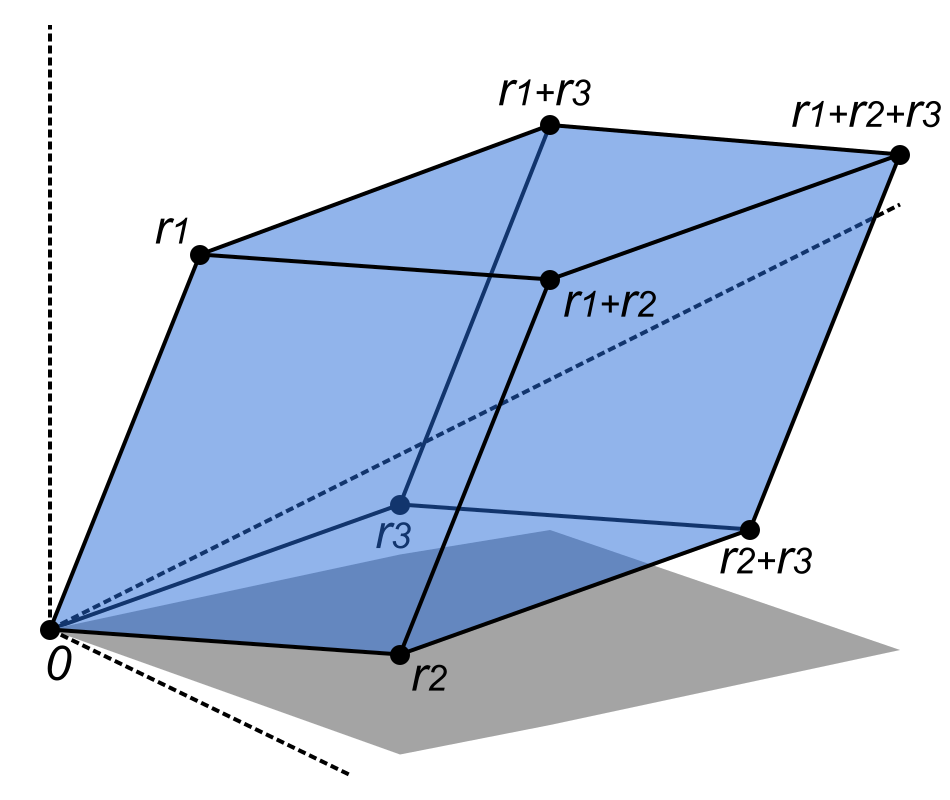
\includegraphics[scale=0.12]{imagens/volume.png}}\\
          \footnotesize{Fonte:~Claudio Rocchini\\ \tiny{(\url{https://en.wikipedia.org/wiki/File:Determinant\_parallelepiped.svg})}}
        \end{center}
      \end{figure}}
    \item Cálculo de \ingles{eigenvalues} (autovalores)
      \only<6>{$$\det(A-\gamma I) = 0$$}
    \item \ldots
  \end{itemize}
\end{frame}

%%%%%%%%%%%%%%%%%%%%%%%%%%%%%%%%%%%%%%%%%%%%%%%%%%%%%%%%%%%%%%%%%%%%%%%%%%%%%%%
%%% Seção: Métodos de cálculo
\section{Métodos de cálculo}

%%% Determinantes 1x1
\begin{frame}[t]
  \frametitle{Determinante de matrizes 1x1}
  \begin{block}{Determinante de matriz 1x1}
    Corresponde ao próprio elemento da matriz:
    \begin{center}
    $\begin{vmatrix}
      a_{11}\end{vmatrix} = a_{11}$
    \end{center}
  \end{block}
\end{frame}

%%% Determinantes 2x2
\begin{frame}[t]
  \frametitle{Determinante de matrizes 2x2}
  \begin{block}{Determinante de matriz 2x2}
    É dado pelo produto dos elementos da diagonal principal, \textbf{menos} o
    produto dos elementos da diagonal secundária:
    \begin{center}
    $\begin{vmatrix}
      a_{11} & a_{12}\\
      a_{21} & a_{22}\end{vmatrix} = a_{11}a_{22} - a_{12}a_{21}$
    \end{center}
  \end{block}
  $\begin{vmatrix}
    \sin{(\theta)} & \cos{(\theta)}\\
    -\cos{(\theta)} & \sin{(\theta)}\end{vmatrix} =$
\end{frame}

%%% Determinantes 3x3
\begin{frame}[t]
  \frametitle{Determinante de matrizes 3x3: Sarrus}
  \begin{block}{Determinante de matriz 3x3}
    Calculamos o determinante pelo \textbf{método de Sarrus}:
    \begin{enumerate}
      \item Repetir as duas primeiras colunas
      \item Calcular a soma do produto das ``diagonais principais''
      \item Calcular a soma do produto das ``diagonais secundárias''
      \item Determinante = $(\text{resultado em } 2) - (\text{resultado em } 3)$
    \end{enumerate}
  \end{block}
  $\begin{vmatrix}
    3 & 2 & -1\\
    1 & -2 & 4\\
    2 & 7 & 5\end{vmatrix}$
\end{frame}

%%% Determinantes 4x4: regra
\begin{frame}[t]
  \frametitle{Determinante de matrizes 4x4: Laplace}
  \begin{block}{Determinante de matriz 4x4}
    Calculamos o determinante pelo \textbf{método de Laplace}:
    \begin{enumerate}
      \item Escolha uma linha ou coluna da matriz com o maior número de
        elementos nulos
      \item Calcule o \textbf{menor complementar} e o \textbf{cofator} de cada
        elemento não nulo da linha ou coluna escolhida
      \item Determinante = $\displaystyle \sum_{k=1}^n (\text{elemento}_k \times \text{cofator}_k)$,
        onde $n$ é o número de elementos não nulos na linha ou coluna escolhida
    \end{enumerate}
  \end{block}
  $\begin{vmatrix}
    3 & 2 & -1 & 0\\
    1 & -2 & 4 & 3\\
    2 & 0 & 3 & 0\\
    -1 & 7 & 5 & 3\end{vmatrix} =$ ?
\end{frame}

%%% Determinantes 4x4: menor complementar
\begin{frame}[t]
  \frametitle{Determinante de matrizes 4x4: Laplace}
  \begin{block}{Menor complementar}
    O \textbf{menor complementar} de um elemento $a_{ij}$ é representado por
    $M_{ij}$ e corresponde ao determinante da matriz resultante ao eliminarmos 
    a linha $i$ e a coluna $j$ correspondentes ao elemento $a_{ij}$ escolhido.
  \end{block}
  $\begin{vmatrix}
    3 & 2 & -1 & 0\\
    1 & -2 & 4 & 3\\
    2 & 0 & 3 & 0\\
    -1 & 7 & 5 & 3\end{vmatrix} =$ ?
\end{frame}

%%% Determinantes 4x4: cofator
\begin{frame}[t]
  \frametitle{Determinante de matrizes 4x4: Laplace}
  \begin{block}{Cofator}
    O \textbf{cofator} de um elemento $a_{ij}$ é representado por
    $C_{ij}$ e é obtido pela fórmula:
  \begin{center}
    $C_{ij} = (-1)^{i+j} \times M_{ij}$
  \end{center}
  \end{block}
  $\begin{vmatrix}
    3 & 2 & -1 & 0\\
    1 & -2 & 4 & 3\\
    2 & 0 & 3 & 0\\
    -1 & 7 & 5 & 3\end{vmatrix} =$ ?
\end{frame}

%%% Determinantes 4x4: finalizando
\begin{frame}[t]
  \frametitle{Determinante de matrizes 4x4: Laplace}
  \begin{block}{Cálculo do determinante}
    Determinante = $\displaystyle \sum_{k=1}^n (\text{elemento}_k \times \text{cofator}_k)$,
        onde $n$ é o número de elementos não nulos na linha ou coluna escolhida
  \end{block}
  $\begin{vmatrix}
    3 & 2 & -1 & 0\\
    1 & -2 & 4 & 3\\
    2 & 0 & 3 & 0\\
    -1 & 7 & 5 & 3\end{vmatrix} =$ ?
\end{frame}

%%% Determinantes 4x4: exemplo completo
\begin{frame}[t]
  \frametitle{Determinante de matrizes 4x4: Laplace}
  $\begin{vmatrix}
    5 & 4 & 1 & 2\\
    -1 & -4 & 2 & 0\\
    3 & 1 & 4 & 0\\
    6 & 1 & 2 & 3\end{vmatrix} =$
\end{frame}


%%%%%%%%%%%%%%%%%%%%%%%%%%%%%%%%%%%%%%%%%%%%%%%%%%%%%%%%%%%%%%%%%%%%%%%%%%%%%%%
%%% Seção: propriedades
\section{Propriedades dos determinantes}

%%% det = 0
\begin{frame}[t]
  \frametitle{Determinante igual a zero}
  As seguintes situações resultam em determinante igual a zero, não importando
  o tamanho da matriz quadrada:
    \begin{enumerate}
      \item Linhas (ou colunas) \textbf{nulas}
        \only<2>{
        $$A = \begin{pmatrix}
          1 & 7 & 3\\
          2 & 9 & 6\\
          0 & 0 & 0\end{pmatrix}
        \quad\quad
        B = \begin{pmatrix}
          1 & 0 & 3\\
          4 & 0 & 9\\
          2 & 0 & 7\end{pmatrix}$$}
      \item Linhas (ou colunas) \textbf{repetidas}
        \only<3>{
        $$A = \begin{pmatrix}
          1 & 7 & 3\\
          2 & 9 & 6\\
          1 & 7 & 3\end{pmatrix}
        \quad\quad
        B = \begin{pmatrix}
          1 & 3 & 3\\
          4 & 9 & 9\\
          2 & 7 & 7\end{pmatrix}$$}
      \item Linhas (ou colunas) \textbf{proporcionais}
        \only<4>{
        $$A = \begin{pmatrix}
          1 & 7 & 3\\
          2 & 9 & 6\\
          3 & 21 & 9\end{pmatrix}
        \quad\quad
        B = \begin{pmatrix}
          1 & 3 & 3\\
          4 & 12 & 9\\
          2 & 6 & 7\end{pmatrix}$$}
      \item Linhas (ou colunas) que são \textbf{combinações lineares} de outras
        duas linhas (ou colunas)
        \only<5>{
        $$A = \begin{pmatrix}
          1 & -2 & 5\\
          5 & -5 & 12\\
          3 & -1 & 2\end{pmatrix}
        \quad\quad
        B = \begin{pmatrix}
          1 & 3 & 4\\
          4 & 12 & 16\\
          2 & 6 & 8\end{pmatrix}$$}
    \end{enumerate}
\end{frame}

%%% Permutação de linhas ou colunas
\begin{frame}[t]
  \frametitle{Permutações de linhas ou colunas}
  \textbf{A cada vez que permutamos} duas linhas (ou duas colunas), o novo
  determinante é o oposto do determinante original (ou seja: o valor absoluto é
  o mesmo, mas \textbf{o sinal é trocado}):
  \only<1->{
  $$A = \begin{pmatrix}
    1 & 2 & 1\\
    2 & 0 & -2\\
    -1 & 3 & 0\end{pmatrix} \implies \det(A) = 16$$}

  \only<2->{
  $$B = \begin{pmatrix}
    2 & 0 & -2\\
    1 & 2 & 1\\
    -1 & 3 & 0\end{pmatrix} \implies \det(B) = -\det(A) = -16$$}

  \only<3->{
  $$C = \begin{pmatrix}
    0 & 2 & -2\\
    2 & 1 & 1\\
    3 & -1 & 0\end{pmatrix} \implies \det(C) = -\det(B) = -(-16) = 16$$}
\end{frame}

%%% Multiplicação escalar de 1 linha ou 1 coluna
\begin{frame}[t]
  \frametitle{Escalar $\times$ uma ÚNICA linha (ou coluna)}
  Se multiplicarmos uma \textbf{única} linha (ou coluna) de uma matriz $A$ por
  um número escalar real $k$, o determinante da matriz $B$ resultante é igual ao
  determinante de $A$ multiplicado por $k$: $\det(B) = k \times \det(A)$:
  \only<1->{
  $$A = \begin{pmatrix}
    1 & 3 & 5\\
    6 & 1 & -2\\
    2 & 4 & -4\end{pmatrix} \implies \det(A) = 174$$}

  \only<2->{
  \begin{equation*}\begin{split}B = \begin{pmatrix}
    1 & 3 & -10\\
    6 & 1 & 4\\
    2 & 4 & 8\end{pmatrix} \implies \det(B) &= -2 \times \det(A)\\
                                           &= -2 \times 174\\
                                           &= -348\end{split}\end{equation*}}
\end{frame}

%%% Multiplicação escalar de todas as linhas
\begin{frame}[t]
  \frametitle{Escalar $\times$ TODAS as linhas}
  Se multiplicarmos \textbf{todas} as linhas (e, por conseqüência, todas as
  colunas) de uma matriz $A$ por um número escalar real $k$, o determinante da
  matriz $B$ resultante é igual ao determinante de $A$ multiplicado por $k$ elevado
  à ordem da matriz: $\det(B) = k^n \times \det(A)$:
  \only<1->{
  \begin{equation*}A = \begin{pmatrix}
    1 & 3 & 5\\
    6 & 1 & -2\\
    2 & 4 & -4\end{pmatrix} \implies \det(A) = 174\end{equation*}}

  \only<2->{
  \begin{equation*}\begin{split}B = \begin{pmatrix}
    -2 & -6 & -10\\
    -12 & -2 & 4\\
    -4 & -8 & 8\end{pmatrix} \implies \det(B) &= (-2)^3 \times \det(A)\\
                                             &= -8 \times 174\\
                                             &= -1392\end{split}\end{equation*}}
\end{frame}

%%% Determinante da transposta
\begin{frame}[t]
  \frametitle{Determinante de uma matriz transposta}
  O determinante de uma matriz transposta $A^t$ é igual ao determinante da
  matriz original $A$ (não transposta):
  \only<1->{
  $$A = \begin{pmatrix}
    1 & 3 & 5\\
    6 & 1 & -2\\
    2 & 4 & -4\end{pmatrix} \implies \det(A) = 174$$}

  \only<2->{
  $$A^t = \begin{pmatrix}
    1 & 6 & 2\\
    3 & 1 & 4\\
    5 & -2 & -4\end{pmatrix} \implies \det(A^t) = \det(A) = 174$$}
\end{frame}

%%% Determinante de matriz triangular/diagonal
\begin{frame}[t]
  \frametitle{Determinante de matriz triangular/diagonal}
  O determinante de uma matriz triangular (superior ou inferior) ou de uma
  matriz diagonal, é igual ao produto dos elementos de sua diagonal principal:
  \begin{equation*}\begin{split}A = \begin{pmatrix}
    2 & 346 & \pi & \sqrt[5]{3}\\
    0 & 9 & -500 & 2^{-189}\\
    0 & 0 & -1 & 432\\
    0 & 0 & 0 & -4\end{pmatrix} \implies \det(A) &= 2 \cdot 9 \cdot (-1) \cdot (-4)\\
                                               &=72\end{split}\end{equation*}
\end{frame}

%%% Teorema de Binet
\begin{frame}[t]
  \frametitle{Teorema de Binet}
  O determinante do produto de duas matrizes é igual ao produto do determinante
  de cada matriz: $\det(AB) = \det(A) \times \det(B)$:
  \only<1->{
  $$A = \begin{pmatrix}
    3 & 1 & 4\\
    1 & 7 & -2\\
    2 & -1 & 5\end{pmatrix} \implies \det(A) = 30$$

  $$B = \begin{pmatrix}
    5 & 0 & 1\\
    1 & 3 & 4\\
    2 & -3 & -2\end{pmatrix} \implies \det(B) = 21$$}

  \only<2->{
  \begin{equation*}\begin{split}AB = \begin{pmatrix}
    24 & -9 & -1\\
    8 & 27 & 33\\
    19 & -18 & -12\end{pmatrix} \implies \det(AB) &= \det(A) \times \det(B)\\
                                                 &= 30 \times 21 = 630\end{split}\end{equation*}}
\end{frame}

%%% Teorema de Jacobi
\begin{frame}[t]
  \frametitle{Teorema de Jacobi}
  Se $B$ for a matriz que resulta quando um múltiplo de uma linha (ou coluna) de
  uma matriz $A$ é somado a uma \emph{outra} linha (ou coluna) de $A$, então
  $\det(B) = \det(A)$:
  \only<1->{
  $$A = \begin{pmatrix}
    3 & 1 & 4\\
    1 & 7 & -2\\
    2 & -1 & 5\end{pmatrix} \implies \det(A) = 30$$}

  \only<2->{
  $$B = \begin{pmatrix}
    5 & 15 & 0\\
    1 & 7 & -2\\
    2 & -1 & 5\end{pmatrix} \implies \det(B) = \det(A) = 30$$}

  \only<3->{
  $$C = \begin{pmatrix}
    3 & 1 & -2\\
    1 & 7 & -4\\
    2 & -1 & 1\end{pmatrix} \implies \det(C) = \det(A) = 30$$}
\end{frame}

%%% Determinante de matriz inversa
\begin{frame}[t]
  \frametitle{Determinante de matriz inversa}
  O determinante de uma matriz inversa $A^{-1}$ é igual ao inverso
  multiplicativo (recíproco) do determinante da matriz $A$ original, ou seja,
  $\det(A^{-1}) = \cfrac{1}{\det(A)}$:
  \only<1->{
  $$A = \begin{pmatrix}
    5 & 0 & 1\\
    1 & 3 & 4\\
    2 & -3 & -2\end{pmatrix} \implies \det(A) = 21$$}

  \only<2->{
  \begin{equation*}\begin{split}A^{-1} = \begin{pmatrix}
    2/7 & -1/7 & -1/7\\
    10/21 & -4/7 & -19/21\\
    -3/7 & 5/7 & 5/7\end{pmatrix} \implies \det(A^{-1}) &= \cfrac{1}{\det(A)}\\ 
                                                        &= \cfrac{1}{21}\end{split}\end{equation*}}
\end{frame}

%%% Determinante da soma
\begin{frame}[t]
  \frametitle{Determinante da soma de matrizes}
  \begin{alertblock}{Cuidado!}
    Em geral o determinante de uma soma de matrizes \textbf{não é} igual à soma
    dos determinantes, ou seja: $$\det(A + B) \ne \det(A) + \det(B)$$
  \end{alertblock}
  \only<1->{
  $$A = \begin{pmatrix}
    2 & -3\\
    4 & 8\end{pmatrix} \implies \det(A) = 28$$

  $$B = \begin{pmatrix}
    5 & 9\\
    -3 & 4\end{pmatrix} \implies \det(B) = 47$$}

  \only<2->{
  $$A+B = \begin{pmatrix}
    7 & 6\\
    1 & 12\end{pmatrix} \implies \det(A+B) = 78$$}
\end{frame}


%%%%%%%%%%%%%%%%%%%%%%%%%%%%%%%%%%%%%%%%%%%%%%%%%%%%%%%%%%%%%%%%%%%%%%%%%%%%%%%
%%% Seção: Chió
\section{Regra de Chió}

%%% Regra de Chió: definição
\begin{frame}[t]
  \frametitle{Regra de Chió}
  Calcula o determinante ``rebaixando'' a ordem da matriz:
  \begin{block}{Regra de Chió}
    \begin{enumerate}
      \item Se o elemento $a_{11}$ da matriz não for unitário, use as
        propriedades dos determinantes para transformá-lo em 1
      \item Elimina-se a primeira linha e a primeira coluna da matriz,
        rebaixando-se assim sua ordem
      \item De cada elemento $a_{ij}$ na matriz rebaixada resultante,
        \textbf{subtrai-se} o produto $a_{i1} \times a_{1j}$
      \item A matriz obtida tem o mesmo determinante que a matriz original
    \end{enumerate}
  \end{block}
  $A = \begin{pmatrix}
    3 & 2 & -1 & 4\\
    1 & -2 & 4 & 0\\
    2 & 7 & 5 & 1\\
    -1 & 2 & 6 & -4\end{pmatrix} \implies \det(A) = $ ?
\end{frame}

%%% Regra de Chió: exemplo
\begin{frame}[t]
  \frametitle{Regra de Chió}
  $A = \begin{pmatrix}
    3 & 2 & -1 & 4\\
    1 & -2 & 4 & 0\\
    2 & 7 & 5 & 1\\
    -1 & 2 & 6 & -4\end{pmatrix}$
\end{frame}


%%%%%%%%%%%%%%%%%%%%%%%%%%%%%%%%%%%%%%%%%%%%%%%%%%%%%%%%%%%%%%%%%%%%%%%%%%%%%%%%
%%% Slide de encerramento com contato (descomentar se necessário)
%\begin{frame}
%\frametitle{Perguntas}
%\begin{center}
%  \Huge ?
%  \vspace{1.6cm}
%  \normalsize
%  \\
%  Abrantes Araújo Silva Filho
%  \\
%  \url{abrantesasf@magister.pro.br}
%  \\
%  \url{https://www.magister.pro.br/}
%\end{center}
%\end{frame}


%%%%%%%%%%%%%%%%%%%%%%%%%%%%%%%%%%%%%%%%%%%%%%%%%%%%%%%%%%%%%%%%%%%%%%%%%%%%%%%%
%%% Encerra a apresentação!
\end{document}
